\documentclass[12pt,letterpaper,oneside]{book}
\usepackage{../afitStyleFiles/afitThesis}
\usepackage{../afitStyleFiles/sf298}
\usepackage{framed,enumitem,graphicx,tikz,tikz-qtree,subfigure}
\usepackage[edges]{forest}
\usepackage{algorithm, pgfplots}
\usepackage[noend]{algpseudocode}

\usetikzlibrary{trees}
\graphicspath{{../Figures/}}
\input{Customize/titlepage}

\makeatletter
\def\BState{\State\hskip-\ALG@thistlm}
\makeatother

\begin{document}

\frontmatter
	\flyleaf                        
	
\mainmatter
\chapter*{Abstract}
In this paper, a novel metaheuristic optimization algorithm named the Leapfrog (LF) metaheuristic is introduced. The proposed metaheuristic takes inspiration from the cheapest insertion construction heuristic and simulated annealing (SA). This paper presents an application of LF to the Traveling Salesman Problem (TSP). To evaluate the efficiency of the proposed algorithm, it was tested using several instances of the TSP using benchmarks from the TSPLIB online library and compared with a similar SA method. The experimental results indicate that the LF metaheuristic is capable of outperforming SA in both runtime and solution quality.
\tableofcontents
\chapter{Introduction}
The Leapfrog Metaheuristic was developed to evaluate a class of NP-Hard problems known as the Travelling Salesman Problem. The TSP consists of a list of cities and distances between them. The goal is to find the shortest tour that visits each city exactly once and returns to the starting city.\\ 
The proposed algorithm utilizes a single-agent hybrid construction/search methodology inspired by aspects of the cheapest insertion construction heuristic and SA. In SA, a local search method is performed to alter a feasible tour and the new tour is accepted with some probability. If the new tour is better than the original one then it is always selected. Otherwise, the probability of selecting the worse solution changes according to some temperature function. The goal of the temperature function is to allow bad solutions to more frequently be selected in the early iterations. Yet as the algorithm continues, the probability of selecting a bad solution decreases. This lets the algorithm escape local minima. This feature of occasionally making bad decisions is used in LF.\\
In the cheapest insertion algorithm nodess are added to a tour under construction such that they are the increase the tour length by the shortest distance. One arc is deleted and the two nodes of that arc are connected to the new node. The problem with this method is that it is deterministic and may easily stop at a suboptimal solution. LF considers a random node, as opposed to the cheapest node, and calculates the cheapest arc to break.\\
Imagine a game of Leapfrog, where one person hops over the back of another person. The people in the game represent the cities in a TSP. Their order represents the tour. Consider the moment when one person leaps. That person is removed from the population and the result is a new tour with one less city. The person then evaluates where to land based on the change in tour distance caused by their insertion at any place in the line. Now consider that multiple people leap at the same time, and one by one they evaluate the best place to return to the line. One round in LF is defined as the leaping and landing of players as described.\\
In LF, the number of people that leap in each round is reduced over the duration of a game as they get tired. A full execution of the algorithm is called a match. A match consists of a selected number of games each consisting of a selected number of rounds. The first round of each game allows the players to choose less than optimal landing spots. This increases the tour length but diversifies the tours being considered in each game.

\chapter{Leapfrog Metaheuristic}
\section{Description}
A match in LF starts by initializing a distance matrix which contains the distance between each pair of nodes. The variable $ n $ is defined as the number of nodes in the map. The user defines the following parameters:
\begin{enumerate}[leftmargin=2.5cm]
	\item[\textbf{players} $ \boldsymbol{p} $] $ \in (0,1]$ This is the maximum ratio of nodes that can be removed during a round. At $ p=1 $, the maximum number of removable nodes, $ n-3 $, are removed. As $ p $ increases the algorithm becomes greedier and run-time increases.
	\item[\textbf{accuracy} $ \boldsymbol{s} $] $ \in (0,1]$ This determines the ratio of possible placements which are considered during the first round of each game. As $ s $ increases, the solution quality decreases (allowing new areas to be explored).
	\item[\textbf{alpha} $ \boldsymbol{a} $] $ \in [0,1]$ This determines the number of players removed during each round. When $ a=0 $, $ p $ players are removed every round. As $ a $ increases, the number of players in each consecutive round decreases at an increasing rate. Run-time also decreases.
	\item[\textbf{length} $ \boldsymbol{r} $] $ \in [1,\infty]$ This is the number of rounds in a game. As $ r $ increases, the depth with which a solution area is explored increases. Run-time also increases.
	\item[\textbf{max} $ \boldsymbol{m} $] $ \in [1,\infty]$ This is the number of games in a match. As $ m $ increases, the diversity of solutions increases. Run-time increases linearly with $ m $.
\end{enumerate}
	A random tour is created by selecting $ n $ nodes with a uniform distribution. The tour is described by a vector containing $ n $ nodes where the order in which the nodes appear represents the order that cities are visited in the tour. The tour is then assumed to return to the first entry in the tour vector. The total distance of this tour is calculated and set as the tour distance. To keep track of the best solution, the current tour and tour distance are set as the best tour and best distance seen so far.\\
	A match consists of $ m $ games ($ j $) each consisting of $ r $ rounds ($ i $). At the beginning of each round, $ i $ is incremented. During the first round of a game ($ i=1 $) the number of nodes to be removed ($ p' $) is calculated using Equation \ref{pprime}.
		\begin{equation}
			p' = \max(p(n-3)e^{-\frac{a(i-1)}{r}},1)
			\label{pprime}
		\end{equation}
	From the current tour, $ p' $ nodes are removed from the tour vector using a random uniform probability. Starting with a random node ($ q $) not in the reduced tour, an arc differential vector is created. The differential vector determines the cost of adding the arc between each pair of remaining $ n-p' $ nodes ($ \boldsymbol{k} $) currently in the tour. The arc differentials are calculated using Equation \ref{arcdiff}.
		\begin{equation}
			\boldsymbol{d}_q = \text{sort}( \text{arc}_{q,k_1}+\text{arc}_{q,k_2}-\text{arc}_{k_1,k_2})\qquad\forall\;k\in \boldsymbol{k}
			\label{arcdiff}
		\end{equation}
	The placement ($ d $) of $ q $ is determined using a random uniform probability and the user defined accuracy parameter in Equation \ref{placement}
		\begin{equation}
		d = UNIF(1,(n-p')s)
		\label{placement}
		\end{equation}
	Placing node $ q $ means inserting $ q $ into the tour vector between the nodes represented by the $ d $th entry in $ \boldsymbol{d}_q $. When $ i>1 $, $ d=1 $. This allows the heuristic to diversify where it is searching at the start of each game then spend time exploring that region for good solutions. This method of exploring the cost differential of every insertion point is repeated for each of the $ p' $ nodes removed from the original tour.\\
	Once all nodes are back in the tour, the tour distance is recalculated. If the tour distance is better than the best seen so far, it is saved as the best tour and best distance. This completes one round.\\
	If the round number ($ i $) equals the game length ($ r $) then set $ i=0 $ and increment the game number ($ j $). This represents the start of a new game. If the max number of games ($ m $) have been played ($ j=m $) then the match is over. At the end of a match, exit the algorithm and return the best tour and best distance found during the match.\\
	Figure \ref{example} steps through a typical round of LF.
	\begin{figure}[H]
		\centering
		\includegraphics[width=.9\linewidth]{example.png}
		\caption{One Round of Leapfrog Metaheuristic on Bays29 Map}
		\label{example}
	\end{figure}
	The neighborhood from one solution to the next is any feasible solution. The neighborhood for any part of the construction phase of LF is restricted to the nodes already in the tour and all but one arc connecting them.
	\section{Tunable Parameters}
	There are several user defined tunable parameters in LF. Any adjustment in the paramters will trade solution quality for runtime. The number of players ($ p $) the game length ($ r $) and the loss rate ($ a $) all work together to determine how greedy the algorithm is during each round. This is shown in Figure \ref{figpprime}.
	\begin{figure}[H]
		\centering
	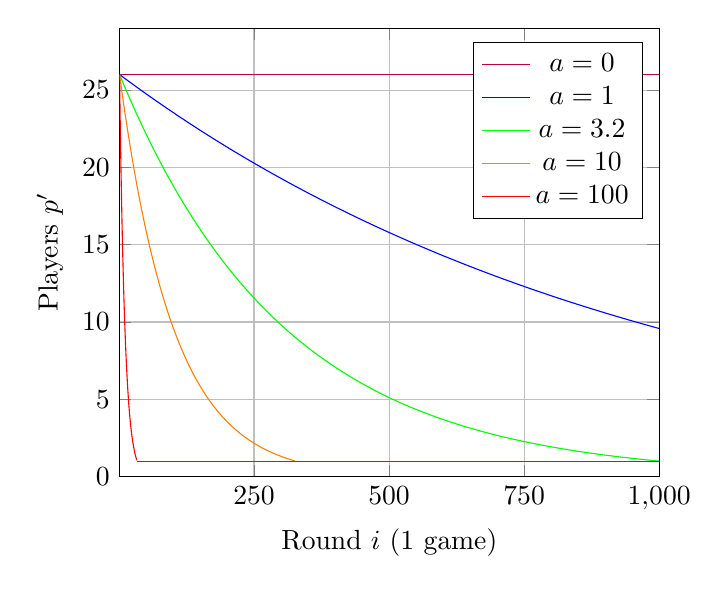
\begin{tikzpicture}
	\begin{axis}[legend pos=north east, grid=major, xmin=1, xmax=1000, ymin=0, ymax=29,
	xlabel=Round $ i $ (1 game), ylabel=Players $ p' $,
	xtick = {250,500,...,1000}, ytick = {0,5,...,25},
	scale=1, restrict y to domain=0.999:29] 
	\addplot[purple, samples=1000, smooth, unbounded coords=discard,domain=1:1000]
	plot (x, { 26*exp((0*(x-1))/1000) });
	\addplot[blue, samples=1000, smooth, unbounded coords=discard,domain=1:1000]
	plot (x, { 26*exp((-1*(x-1))/1000) });
	\addplot[green, samples=1000, smooth, unbounded coords=discard,domain=1:1000]
	plot (x, { 26*exp((-3.26*(x-1))/1000) });
	\addplot[orange, samples=1000, smooth, unbounded coords=discard,domain=1:1000]
	plot (x, { 26*exp((-10*(x-1))/1000) });
	\addplot[red, samples=1000, smooth, unbounded coords=discard,domain=1:1000]
	plot (x, { 26*exp((-100*(x-1))/1000) });
	\addplot[red, samples=1000, smooth, unbounded coords=discard,domain=33.5:1000]
	plot (x, { 1*exp((0*(x-1))/1000) });
	\legend{$a=0$,$a=1$,$ a=3.2 $,$a=10$,$a=100$}
	\end{axis}
	\end{tikzpicture}
	\caption{Effect of $ \boldsymbol{a} $ on $ \boldsymbol{p'} $ for Bays29 with $ \boldsymbol{p=1} $}
	\label{figpprime}
	\end{figure}
\noindent Figure \ref{tblparams} discusses the pros and cons of changing the values for each parameter. The run-time has a direct linear relationship to $ r $ and $ m $. The following settings were found to balance run-time with solution quality when the number of cities in an instance was less than 150.
 \[p=1\quad s=0.5\quad a=10\quad r=100\quad m=10\]
As the instance size grows, the computational time scales non-linearly. A reduction of $ m,\;r $, or $ p $, or an increase in $ a $, may lead to worse solutions but will decrease the run-time.
\begin{figure}[H]
	\centering
	\begin{tabular}{|c|l|l|}
		\hline
		Parameter&Lower&Higher\\
		\hline
		$ p $&less greedy, faster&greedier, slower\\
		$ s $&less diversification&more diversification\\
		$ a $&greedier, less intensification, slower&less greedy, more intensification, faster\\
		$ r $&less intensification, faster&more intensification, slower\\
		$ m $&less diversification, faster&more diversification, slower\\
		\hline
	\end{tabular}
	\caption{Parameter Effects Comparison Table}
	\label{tblparams}
\end{figure}
\noindent Figure \ref{params} shows a tour's objective value plotted over a complete match. Each parameter's general effect is marked. The steepness of the slope at first is related to the greediness of the heuristic and is a result of a high $ p $. The steep intensification line without bottoming out shows that $ a $ and $ r $ are too low. The height of each diversification jump shows that each game is played in a sufficiently diverse region of the solution space.
	\begin{figure}[H]
		\centering
		\includegraphics[width=1\linewidth]{params.png}
		\caption{Parameter Effects on Objective Value}
		\label{params}
	\end{figure}
LF also works extremely well as a single iteration construction heuristic. Running the algorithm against the map pr1002 (with the parameters: $ p=1,\;s=0.01,\;a=0,\;r=1,$, and  $m=1 $) yielded the following solution within two seconds. The greedy solution had an 11\% relative error from the optimal solution. Figure \ref{oneshot} shows the initial random solution and the final one-iteration greedy solution.
 \begin{figure}[H]
 	\centering
 	\includegraphics[width=.85\linewidth]{oneshotbefore.png}
 	\includegraphics[width=.85\linewidth]{oneshotafter.png}
 	\caption{Single Iteration Construction Heuristic Results}
 	\label{oneshot}
 \end{figure}
\section{Pseudocode and Flowchart}
The main steps of LF are summarized in Algorithm \ref{pseudo} and in the flowchart in Figure \ref{flow}.
	\begin{algorithm}[H]
		\caption{Leapfrog Metaheuristic}
		\label{pseudo}
		\begin{algorithmic}[1] 
			\State \textbf{Initialize} map, players $ (p) $, accuracy $ (s) $, length $ (r) $, max $ (m) $, alpha $ (a) $
			\State \textbf{set} $ n= $ number of nodes on map, $ i=0 $, $ j=0 $
			\State \textbf{generate} random tour using $ UNIF(1,n) $
			\State \textbf{calculate} tour distance
			\State \textbf{set} best tour = tour, best distance = tour distance
			\While {$ j < m $}
			\State $ i++ $, $ p' = \max(p*(n-3)*e^{-\frac{a(i-1)}{r}},1) $
			\State Remove $ p' $ nodes randomly from tour
			\For {all removed nodes}
			\State Calculate and rank the cost of adding between each node in tour
			\If {i = 1}
			\State Place node in ranked arc $ UNIF(1,(n-p')*s) $
			\Else
			\State Place jumpers in ranked arc 1
			\EndIf
			\EndFor
			\State Calculate tour distance
			\If {tour distance $ < $ best distance}
			\State best tour = tour, best distance = tour distance
			\EndIf
			\If {i = r}
			\State i = 0, j++
			\EndIf
			\EndWhile
		\end{algorithmic}
	\end{algorithm}

\begin{figure}[h]
	\centering
	\includegraphics[width=1\linewidth]{flow.png}
	\caption{Leapfrog Heuristic Flowchart}
	\label{flow}
\end{figure}


\chapter{Computational Results}
\section{Test Description}
An instance of SA, similar to LF, was created to test LF's performance. Since both algorithms are single agent local search heuristics, this choice is appropriate. LF is greedier than SA and its run-time is determined by the number of iterations it is instructed to perform. Therefore, it is not adequate to simply run the two methods for the same number of iterations as this would bias the analysis heavily in favor of LF because of its ability to get decent solutions after a single iteration. Instead, LF was run for 20 trials on each of 13 instances of the TSP and the SA algorithm was allowed to operate for the same duration of time as LF for every replication. This created a method to compare solution quality while controlling for computational effort.
\section{Run-time}
For each of the 11 of the 13 maps, the initial run-time was determined by applying LF with the parameters:
\[p=1\quad s=0.5\quad a=10\quad r=100\quad m=10\]. To show how these parameters can be changed to alter the run-time and solution quality, the parameters for the maps with 343 and 1002 nodes were set to: 
\[p=1\quad s=0.5\quad a=10\quad r=50\quad m=5\]\\
It is clear from Figure \ref{rt} that the change brought down the time substantially for the map with 343 nodes. For the map with 1002 nodes, the original parameters resulted in a run-time of nearly twenty minutes but a relative error of only three percent. Thus, the run-time was reduce by ninety percent but the relative error was worsened by five percent. These run-times were the exit criteria for each identical instance of the SA algorithm.
\begin{figure}[H]
	\centering
	\includegraphics[width=1\linewidth]{rt.png}
	\caption{Run-time vs Node Count}
	\label{rt}
\end{figure}

\section{Relative Error}
The relative error of a solution was calculated using Equation \ref{req}
\begin{equation}
	RE (\%)=100\left(\dfrac{\text{best distance}-\text{optimal distance}}{\text{optimal distance}}\right)
	\label{req}
\end{equation}
Figure \ref{re} shows the relative error recorded for each of the two algorithms. The optimal solution was found by LF for all six instances with 100 nodes or less. In three of those cases, LF only returned the optimal solution.\\
On the map with 343 nodes, both the solution time and the solution quality were improved over the map with 225 nodes. This suggests that a better tuning strategy should be investigated.\\
In every single replication, LF outperformed SA. The solutions were shown to follow an approximately normal distribution and there was no statistical overlap of a 95\% confidence interval on the relative error of the SA and LF solutions, except in the instance with 225 nodes.
\begin{figure}[H]
	\centering
	\includegraphics[width=1\linewidth]{re.png}
	\caption{Relative Error vs Node Count}
	\label{re}
\end{figure}
The solutions produced by SA have more variance than those from LF. In every case tested, LF produced more consistent results than SA. A table of the best results for each metaheuristic is shown in Figure \ref{table}.
\begin{figure}
	\centering
	\resizebox{1 \textwidth}{!}{
	$\begin{array}{|c|ccccccccccccc|}
		\hline
		\text{Node Count}&29&48&51&52&76&100&120&130&195&225&343&442&1002\\
		\hline
		\text{Time (s)}&5.739&8.910&9.455&9.481&12.826&16.852&23.718&23.767&31.717&67.937&30.856&70.303&144.206\\
		\text{Optimal}&2020&5046&426&7542&108159&21282&6942&6110&2323&126643&1368&50778&259045\\
		\hline
		\text{LF}&2020&5046&426&7542&108159&21282&6990&6126&2399&128056&1399&52816&279197\\
		\text{LF Err \%}&0&0&0&0&0&0&0.69&0.26&3.27&1.12&2.27&4.01&7.78\\
		\hline
		\text{SA}&2159&5274&475&8258&112590&24411&7518&6465&2548&128525&1564&58897&340082\\
		\text{SA Err \%}&6.88&4.52&11.50&9.49&4.10&14.70&8.30&5.81&9.69&1.49&14.33&15.99&31.28\\
		\hline
	\end{array}$
	}
\caption{LF vs SA Comparison Data}
\label{table}
\end{figure}
\section{Further Research}
There are many opportunities to improve upon LF. In its current form, there is no memory function. It may be useful to develop tabu lists for arcs. This would greatly increase diversify and counteract the greediness of the algorithm but may slow down each differential calculation.\\
Another potential use for memory would be to search a few diverse solutions with a high number of players, then intensify on the best few with many rounds consisting of only a few players. This would increase the computational complexity in the first few rounds of each game. The intensification stage in this scenario would have a high $ r $ and $ a $, which reduces the computational complexity of the later rounds in a game.\\
The tunable parameters also offer an opportunity to develop a combinatorial problem. The parameters chosen in this paper were developed by running the algorithm, plotting the results, and slowly changing them until good solutions were produced faster and more often. The map with 323 nodes demonstrated the capacity for better tuning of the parameters.\\
The shape of the map affects the solution as much as the number of nodes. There may be a benefit to deciding which nodes will not be removed during each iteration and the order in which nodes are added back in. This predetermined method could potentially allow the algorithm to construct better solutions but may become prey to local minima.\\
The equation to determine the number of nodes removed each round reduces very quickly. It may be wise to emplement a step-wise function that allows for more solutions that are greedy early on but then settles on a spot and runs many more single node solutions since they are much faster. This would create more intensification without substantially affecting the computational effort.\\
The distance look-up matrix is a major source of computational waste. An implementation of a k-d tree may speed up the development of the differential vector.

\chapter{Conclusions}
In this paper, a novel metaheuristic optimization algorithm named the Leapfrog Metaheuristic was introduced. The proposed metaheuristic was evaluated on several instances of the TSP using benchmarks from the TSPLIB online library and compared with a similar SA method.\\
The experimental results indicate that LF is capable of outperforming SA in both runtime and solution quality. The algorithm was also shown to be tunable to operate as a single-iteration construction heuristic which returns better solutions than the nearest neighbor heuristic.\\
Although LF performed the best in this evaluation, there are still a lot of improvements to be made. Better tuning of the parameters may reduce the computational time required and improve the solution quality. A thorough regression analysis would provide insight into the trade-off limitations between solution quality and computational complexity.\\
One thing is certain from this analysis: if the exact optimal answer is not required then the Leapfrog Metaheuristic is well suited to find an acceptable solution in the shortest time.

\end{document}
